\documentclass[11pt]{article}
\usepackage{enumerate,fancyvrb,graphicx}
\usepackage[utf8x]{inputenc}
\usepackage{fullpage}
\linespread{1.25}

\begin{document}
\title{The Inkboard protocol specification}
\author{David Yip}
\maketitle

\begin{abstract}
Inkboard is a component of the Inkscape vector graphics editor that allows Inkscape users to collaborate on Inkscape documents.  This document describes the protocol used by Inkboard clients to manage sessions, communicate document changes, and resolve conflicting changes.
\end{abstract}

\tableofcontents

\section{Introduction}
\subsection{Overview}
Inkboard is a component of the Inkscape vector graphics editor that allows Inkscape users to collaborate on Inkscape documents.  The protocol is implemented as a layer on top of the XMPP instant-messaging protocol\cite{rfc3920}, which is the core of the Jabber instant-messaging system.

\subsection{Terminology}
The capitalized key words "MUST", "MUST NOT", "REQUIRED", "SHALL", "SHALL NOT", "SHOULD", "SHOULD NOT", "RECOMMENDED", "MAY", and "OPTIONAL" in this document are to be interpreted as described in BCP 14, RFC 2119\cite{rfc2119}.

\section{Definitions}
The following definitions are used throughout this document.
\begin{itemize}
\item {\em Inkboard user}: The user of an Inkboard client.  
\item {\em Inkboard change}: An XML fragment specifying a change to be made to a document.  A full listing of change types is given in Section \ref{change-types}.
\item {\em User-to-user session}: An Inkboard session only occurring between two users.  Analogous to traditional text-based instant messaging between two users.
\item {\em User-to-conference session}: An Inkboard session occurring between a user and a multi-user conference room.  Analogous to traditional text-based chat rooms.
\end{itemize}

\subsection{Dramatis Personae}
Throughout this document, references will be made to the following fictional entities:
\begin{center}
\begin{tabular}[t]{|c|c|}
\hline
Entity Name & Role \\
\hline
Romeo & Inkboard user \\
\hline
Juliet & Inkboard user \\
\hline
Chat & Conference room \\
\hline
\end{tabular}
\end{center}

\section{A brief overview of the Inkboard architecture}
Because the Inkboard protocol is heavily influenced by the architecture of the Inkboard component, a brief overview of Inkboard's architecture may be helpful in understanding the Inkboard protocol.

Inkboard is implemented as a listener attached to the Inkscape undo/redo mechanism.  Inkscape maintains one undo log and one redo log per document.  Inkscape undo log listeners receive notifications on the following events:

\begin{enumerate}
\item An undo action was requested by the user.
\item A redo action was requested by the user.
\item A set of changes was committed to the undo log.
\end{enumerate}

When any of these events occur, the Inkboard undo listener receives a pointer to an object of type \texttt{Inkscape::XML::Event}, which represents manipulations on the XML tree representing an SVG document.  The Inkboard undo listener serializes these \texttt{Inkscape::XML::Event} objects into Inkboard changes and then sends them out to the recipient.

The receiving Inkboard client attempts to deserialize these messages into \texttt{Inkscape::XML::Event} objects.  If deserialization is successful, these \texttt{Inkscape::XML::Event} objects are replayed using the Inkscape undo mechanism.

\section{Inkboard and XMPP}
\subsection{Format of Inkboard messages}
Inkboard messages are encapsulated in XMPP message stanzas, the format of which is described in \cite{rfc3920}.  Inkboard data is wrapped in an \texttt{<inkboard>} element which MUST contain the following attributes:
\begin{center}
\begin{tabular}[t]{|c|c|}
\hline
Attribute & Description \\
\hline
\texttt{protocol} & Version of the Inkboard protocol utilized by the client that sent the message.\\
& Clients conforming to this specification MUST use version number 2 in this field. \\
\hline
\texttt{type} & Numeric identifier of a message type. \\
&  See Section \ref{message-types} for a full listing of Inkboard message types. \\
\hline
\texttt{seq} & Sequence number of the message.  This MUST be monotonically increasing.  \\
\hline
\end{tabular}
\end{center}

Inkboard changes MUST be wrapped inside an \texttt{<x:inkboard-data>} element inside the \texttt{<inkboard>} element.  The \texttt{<x:inkboard-data>} tag MUST contain zero or more Inkboard changes.  See Section \ref{example-messages} for examples of Inkboard messages, and Section \ref{change-types} for a full listing of Inkboard change types.

The Inkboard XML schema is available at \texttt{http://inkscape.org/inkboard}.  

\subsection{Inkboard message queuing rules}
Inkboard messages MUST be processed as soon as possible (i.e. as soon as they are received), with the sole exception of Inkboard messages of type \texttt{CHANGE}.

Inkboard messages of type \texttt{CHANGE} SHOULD NOT be applied to a document as they are received; instead, Inkboard clients SHOULD queue up changes until receipt of a \texttt{COMMIT} message.  Upon receipt of a \texttt{COMMIT} message from a particular Inkboard client, Inkboard clients implementing the queuing method MUST commit all uncommitted changes received from that particular client.

\subsection{Example Inkboard messages}
\label{example-messages}
\subsubsection{Null message}
\VerbatimInput[tabsize=2]{inkboard-message-examples/null-message.txt}

\subsubsection{Sending a change}
\VerbatimInput[tabsize=2]{inkboard-message-examples/1-1-change-message.txt}

\section{Session establishment}
\subsection{User-to-user}
User-to-user sessions MUST be negotiated according to the procedure outlined below.

\begin{figure}
\label{u2u-session-establishment-figure-accept}
\centering
\includegraphics[width=5in]{eps/session-invite-u2u-01.eps}
\caption{Initiation of an Inkboard session between two users.}
\end{figure}

\begin{figure}
\label{u2u-session-establishment-figure-reject}
\centering
\includegraphics[width=5in]{eps/session-invite-u2u-02.eps}
\caption{Attempt to initiate an Inkboard session between two users, with the second user rejecting the invitiation.}
\end{figure}

\begin{enumerate}
\item Romeo invites Juliet to a user-to-user session using his Inkboard client. 
\item Romeo's Inkboard client sends a \texttt{CONNECT\_REQUEST\_USER} message to Juliet's Inkboard client.
\item Juliet's Inkboard client notifies Juliet that Romeo has invited her to a user-to-user session.
\begin{enumerate}
\item If Juliet accepts Romeo's invitation:
\begin{enumerate}
\item Juliet's Inkboard client sends a \texttt{CONNECT\_REQUEST\_RESPONSE\_USER} message to Romeo's Inkboard client.
\item Romeo's Inkboard client notifies Romeo that Juliet has accepted his invitation.
\item Romeo's Inkboard client sends a \texttt{CONNECTED\_SIGNAL} message to Juliet's Inkboard client.
\item Romeo's Inkboard client serializes the current contents of Romeo's SVG document.
\item Romeo's Inkboard client sends a \texttt{DOCUMENT\_BEGIN} message to Juliet's Inkboard client.
\item Romeo's Inkboard client sends the serialized document to Juliet's Inkboard client as a series of \texttt{CHANGE} messages.
\item Romeo's Inkboard client sends a \texttt{COMMIT} message to Juliet's Inkboard client.
\item Upon receipt of Romeo's \texttt{DOCUMENT\_BEGIN} message, Juliet's Inkboard client prepares to process incoming \texttt{CHANGE} messages from Romeo's Inkboard client by doing the following actions:
\begin{enumerate}
\item Juliet's existing document is cleared.
\item Juliet's Inkboard client prepares to receive and process incoming \texttt{CHANGE} messages.
\end{enumerate}
\item Upon receipt of Romeo's \texttt{COMMIT} message, Juliet's Inkboard client commits all changes sent by Romeo's Inkboard client.
\end{enumerate}
\item If Juliet rejects Romeo's invitation:
\begin{enumerate}
\item Juliet's Inkboard client sends a \texttt{CONNECT\_REQUEST\_REFUSED\_BY\_PEER} message to Romeo's Inkboard client.
\item Romeo's Inkboard client notifies Romeo that Juliet refused his invitation.
\end{enumerate}
\end{enumerate}
\end{enumerate}

\subsubsection{Example of accepted invitation}

\subsubsection{Example of rejected invitation}

\subsection{User-to-conference}
User-to-conference sessions MUST be negotiated according to the procedures outlined below.

The procedure for user-to-conference session establishment differs based on whether or not there already exist Inkboard users in a Jabber conference room; therefore, there are two modes of operation for Inkboard clients.  These two modes are dubbed {\em synchronization mode}, in which an Inkboard client synchronizes with the rest of the conference, and {\em transceiver mode}, in which an Inkboard client transmits and receives changes to/from all other conference members.  The presence of other Inkboard users is determined by the following rules:

\begin{enumerate}
\item If the user joining a user-to-conference session is the only member of the conference, then that user's Inkboard client SHOULD assume that it is the first participant in a chatroom and immediately enters transceiver mode.
\item If the user joining a user-to-conference session is not the only member of the conference, then that user's Inkboard client MUST enter synchronization mode.  See Section \ref{joining-existing-conference} for synchronization mode procedures.
\end{enumerate}

Room rosters MUST be processed according to the procedures given in Section 6.3.3 of \cite{jep0045}.

\begin{figure}
\label{u2c-session-establishment-figure-accept}
\centering
\includegraphics[width=5in]{eps/session-invite-u2c-01.eps}
\caption{Initiation of an Inkboard session between a user and a conference in which Inkboard users are already involved in a conference.}
\end{figure}

\subsubsection{User establishing a new conference}
\begin{enumerate}
\item 
\end{enumerate}

\subsubsection{User joining an existing conference}
\label{joining-existing-conference}
\begin{enumerate}
\item 
\end{enumerate}

\section{Session establishment error cases}
\subsection{Incompatible protocol versions}

\subsubsection{User-to-user}

\subsubsection{User-to-conference}

\subsection{Duplicate session establishment requests}

\subsection{Mutual invitation}

\section{Transmitting changes}
\subsection{User-to-user}

\subsection{User-to-conference}

\section{Change conflict resolution}

\section{Client requirements}
[describe what is required of a client implementing this protocol; this will probably need to delve into the Inkscape document model a little bit]

\section{Contributors}
[TBW]

\section{Acknowledgments}
[TBW]

\section{Security considerations}
[TBW]

\section{IANA Considerations}
[TBW, although most likely ``None'']

\appendix
\section{Appendices}

\subsection{Full listing of message types}
\label{message-types}

\subsection{Full listing of change types}
\label{change-types}

\bibliographystyle{alpha}
\bibliography{protocol.bib}

\end{document}